\subsection{TCP measurements}\label{sec_tcp_mes}


\subsection*{Purpose:}

The purpose is to determine the maximum frequency that can be used with the TCP/IP protocol.  To do so, Wireshark is used to record information about the traffic. The values that are necessary for analyzing the connection are the delay between two packets received or sent and from that, the actual frequency as it may differ from the value programmed, the jitter and the packet loss. 
\subsection*{Test equipment:}

The sbRIO 9636 is connected to a computer running Ubuntu 14.04 LTS via an Ethernet cable of 1 gpbs. The computer runs the ROS nodes that are used for the project, thus it communicates with both the Geomagic Touch and the sbRIO and it sends random setpoints to the sbRIO. The sbRIO uses the entire code of the project.

\subsection*{Procedure:}

\begin{enumerate}
	\item The sbRIO is started and connected to the computer.
	\item The ROS node is started.
	\item Wireshark is started.% using this command: tshark -i 1 -f tcp -a duration:20 -w ~/wireshark_capture
	\item Once the recording is done the ROS node is stopped. The recording time here was 20 seconds.
	\item The log files are retrieved to be analyzed using Matlab and Wireshark.
\end{enumerate}
Those steps are repeated for the following settings: 100Hz, 500Hz and 1000Hz.


\subsection*{Measuring data:}

	\begin{figure}[h]
		\centering
		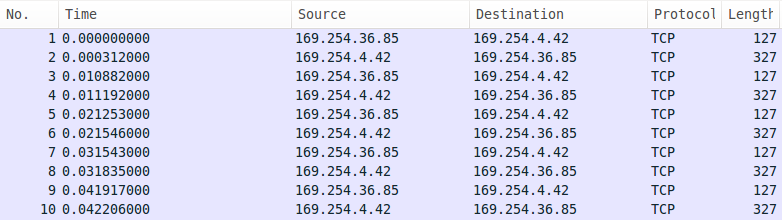
\includegraphics[width=\linewidth]{10ms_TCP.png}
		\caption{Wireshark recordings for 100Hz}
		\label{fig:10ms_tcp}
	\end{figure}
	\begin{figure}[h]
		\centering
		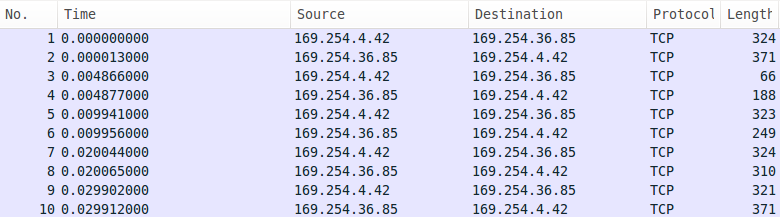
\includegraphics[width=\linewidth]{2ms_TCP.png}
		\caption{Wireshark recordings for 500Hz}
		\label{fig:2ms_tcp}
	\end{figure}
	\begin{figure}[h]
		\centering
		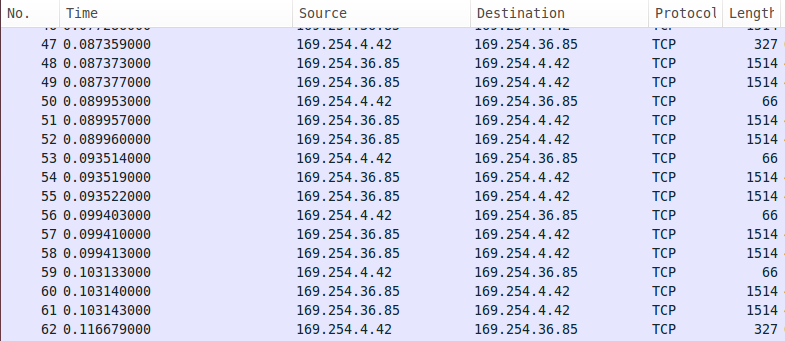
\includegraphics[width=\linewidth]{0ms_TCP.png}
		\caption{Wireshark recordings for 1000Hz}
		\label{fig:0ms_tcp}
	\end{figure}

% \begin{center}
% 	$\begin{tabular}{c|ccccc}
% 		\text{Delay} & \text{Sending\newline frequency (Hz)} & \text{Receiving frequency (Hz)} & \text{Average delay (ms)} & \text{Jitter} & \text{Error rate (\%)}\\
% 		\hline
% 		10ms & 4 & 4 & 1 & 1 & 1 \\
% 		2ms & 4 & 4 & 1 & 1 & 1 \\
% 		0ms & 1 & 1 & 1 & 1 & 15 \\
% 	\end{tabular}$
% 	\captionof{table}{TCP}
% \end{center}

\subsection*{Results:}

When the frequency is increased above 100Hz, instead of sending more packets it sends bigger packets in which two \gls{JSON} files or more are grouped. As shown on \figref{fig:10ms_tcp}, \figref{fig:2ms_tcp}, \figref{fig:1ms_tcp}, the more the frequency is increased, the bigger the packets. 

\subsection*{Conclusion:}

The communication does not have the desired behavior when the frequency is increased. Thus the jitter and packet loss cannot be used to evaluate the performance. This may be due to the default behavior of TCP or to the default behavior of the JSON Stream. It was decided not to look further into this subject as this problem does not appear in the new communication protocol since it does not implement any connection or stream.